%!TEX root = Manuscript.tex

%解释DSM,DoD,GCP,multi-epoch, intra and inter epoch, GT
\chapter{Introduction}
\label{chap:intro}
\minitoc

\section{Motivation}
\subsection{Why are historical images interesting}
Historical (i.e. analogue or archival) aerial images play an important role in providing unique information about evolution of land-covers. 
They are objective witness over time and sometimes the only remaining visual source of historical land-form. Therefore, they are valuable assets for a wide range of applications such as: (1) change detection, (2) spatial and urban planning, (3) long-term environmental monitoring including but not limited to forests, ice glaciers and coastlines, (4) analysis of natural disaster (e.g. earthquake, volcano eruption, landslide ect.) and the estimation of its future trends, etc.
%用途:地震,冰川,土地规划?
%long-term environmental monitoring: forests, ice glaciers, coastlines etc.
%change detection; 
%spatial and urban planning, boundary disputes, etc.
%enable the analysis of natural disaster (e.g. earthquake, volcano eruption, landslide ect.) and the estimation of its future trends.
\par
Historical aerial images have regularly been acquired since the 1920’s by mapping, military or cadastral agencies all over the world. A mass amount of them have been digitized and made accessible through web services~\cite{sebastien2019archiving,earthexplorer,remonterletemps}. 
For example, according to a survey in Europe~\cite{sebastien2019archiving}, there are in total 50 million of aerial images archived, with around 37.8\% of them digitized.
%A survey called "State of current practices concerning archival aerial images" in Europe~\cite{sebastien2019archiving} took place in 2017, 19 organizations from 13 countries (including Austria, Norway, Finland, Spain, Slovenia, Cyprus, Czech Republic, Finland, Germany, Switzerland, Sweden, Poland, France and United Kingdom) replied. According to it, there are in total 50 million of aerial images archived, with around 37.8\% of them digitized.
The images are of high spatial resolution, and are acquired in stereoscopic configuration, allowing for 3D restitution of territories. 
They are often accompanied by metadata, in most cases including the camera focal length and the physical sensor size. Other metadata such as flight plans, camera calibration certificates or orientations are not commonly available. 
\par
When the camera calibration parameters are unknown, they should be evaluated by a process called self-calibrating bundle adjustment. Adequate Ground Control Points (\ac{GCP}s) are required, otherwise inaccurately estimated camera parameters will lead to systematic error surfaces called dome effect (i.e. bowel effect).
Generally, \ac{GCP}s originate from (i) field surveys \cite{micheletti2015application,walstra2004time,cardenal2006use}, (ii) recent orthophotos and DEM \cite{nurminen2015automation,ellis2006measuring,fox2008unlocking} and (iii) recent satellite images \cite{ellis2006measuring,ford2013shoreline}. The most challenging part is to identify the \ac{GCP}s on the historical images, due to inevitable scene changes. \ac{GCP}s are usually manually measured with the help of recent photos, however, it is still monotonous and time-consuming. 
There is an urgent need to automatically identify corresponding points (i.e. matches) on historical and recent images.\\
When users are only interesting in comparing different historical epochs, the self-calibration can be accomplished without \ac{GCP}s. Matches between different epochs would serve as observations in bundle adjustment to eliminate the dome effect between surfaces from different epochs. In conclusion, the bottleneck of historical image self-calibration located in recovering matches on images taken at different times (i.e. multi-epoch).
%困难:
%(1) 数据异构: images exhibit highly heterogeneous spatial resolutions, with very different acquisition conditions (season, sensors etc.); 
%(2) camera's parameters  may not be available as they might  be  lost  during  the  years  or  never documented; inappropriate film/glass plate preservation; deformation due to scanning process; 
%(3)Drastic scene changes
%(4)Low radiometric quality: old-fashioned radiometric characteristics; noisy; even scratchs on the original films; deterioration due to the aging of the film

%Corresponding points 
%Besides, inappropriate film/glass plate preservation and the scanning process enforce reestimating of the camera calibrations (i.e., the self-calibrating).\\

\subsection{How to match multi-epoch historical images}
However, matching multi-epoch historical images remains challenging, despite the fact that there exists a large number of image matching algorithms with their effectiveness proven on modern images, for the following reasons:
\begin{itemize}
	\item Multi-epoch images are often acquired at different times of day and in different weathers or seasons, which unavoidably leading to appearance differences.
	\item The scene changes over time due to anthropogenic phenomenas (e.g. urban planning) or natural ones (e.g. earthquake), especially for large time gaps.
	\item Multi-epoch images often exhibit heterogeneous spatial resolutions, accompanied with different acquisition conditions (sensors, spectral channels, etc.).
	\item Historical images are often facing low radiometric quality, including low contrast, image noise, deterioration due to the aging of the films, or even scratches on the films.
\end{itemize}

\subsubsection{Take advantage of 3D geometry}
The key idea of our method is to use 3D geometry to guide matching. This idea comes from the observation that RGB images have the following shortcomings:\\
(1) Their appearances change over time (see Figure~\ref{AppearanceChange}), and with varying view angles on non-Lambertian surfaces (see Figure~\ref{PoorlyTextured}).\\
(2) Self similarities (e.g. repetitive patterns) favor false matches (see Figure~\ref{PoorlyTextured}).\\

\begin{figure*}[htbp]
	\begin{center}
		\subfigure[Image 1971]{
			\begin{minipage}[t]{0.45\linewidth}
				\centering
				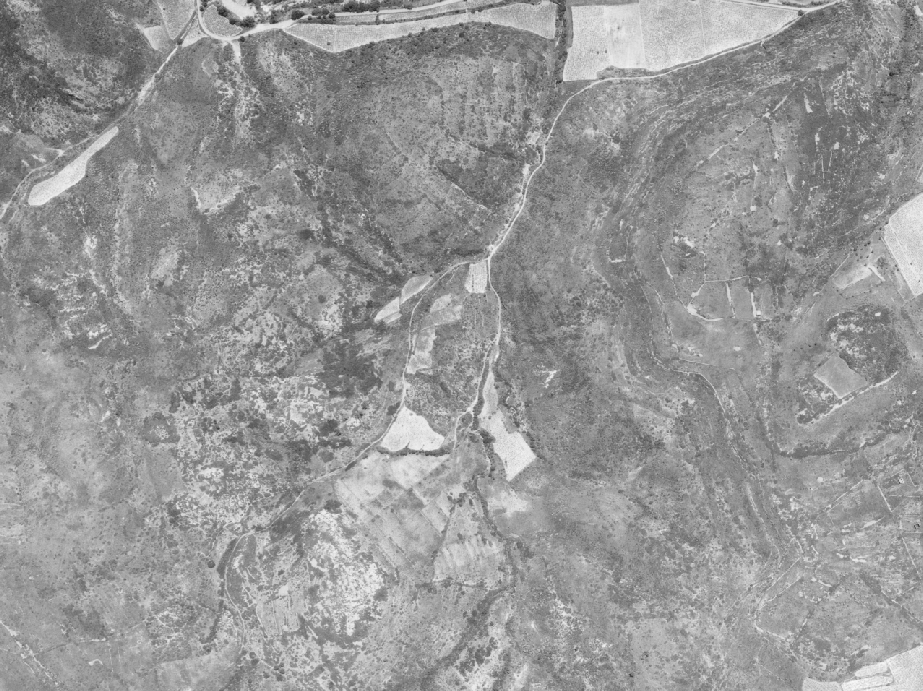
\includegraphics[width=6.2cm]{images/Chapitre1/AppearanceChangeRGBL.png}
			\end{minipage}%
		}
		\subfigure[Image 2015]{
			\begin{minipage}[t]{0.45\linewidth}
				\centering
				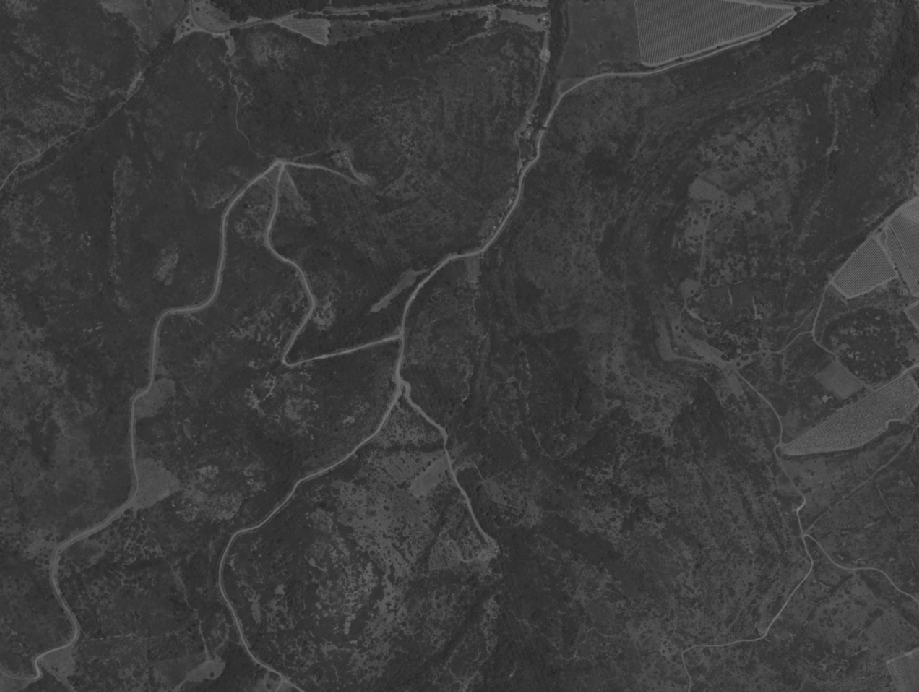
\includegraphics[width=6.2cm]{images/Chapitre1/AppearanceChangeRGBR.png}
			\end{minipage}%
		}
		\subfigure[\ac{DSM} 1971]{
			\begin{minipage}[t]{0.45\linewidth}
				\centering
				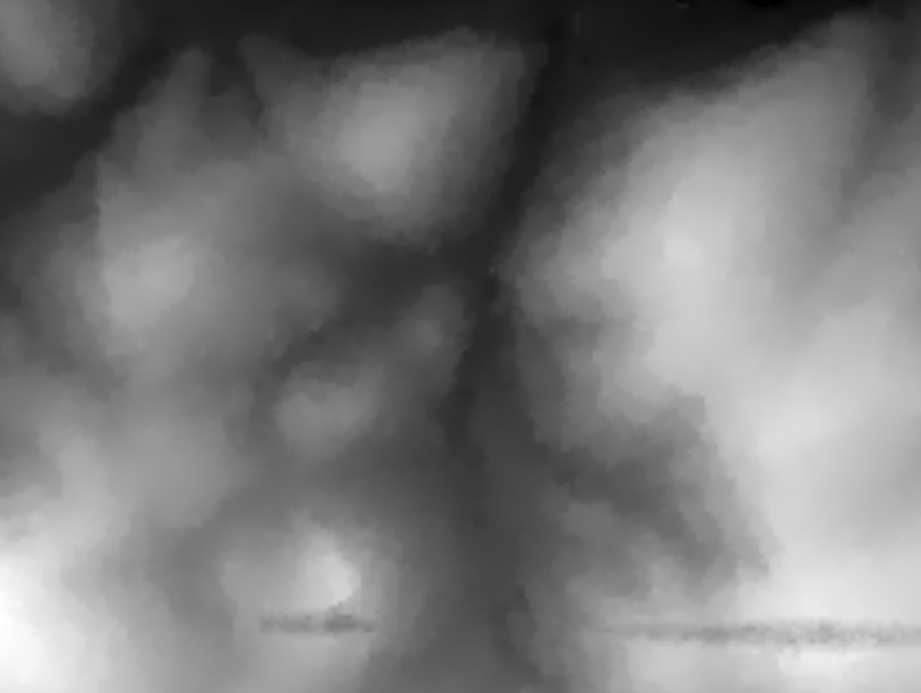
\includegraphics[width=6.2cm]{images/Chapitre1/AppearanceChangeDSML.png}
			\end{minipage}%
		}
		\subfigure[\ac{DSM} 2015]{
			\begin{minipage}[t]{0.45\linewidth}
				\centering
				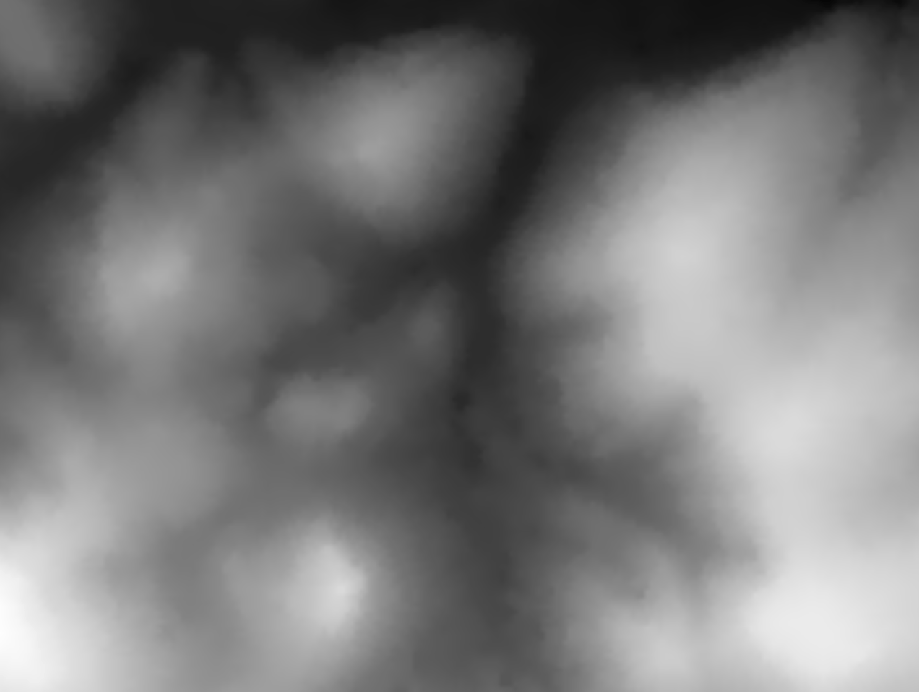
\includegraphics[width=6.2cm]{images/Chapitre1/AppearanceChangeDSMR.png}
			\end{minipage}%
		}
		\caption{The same zone observed in different times. The images changed a lot while the \ac{DSM}s stayed stable over time.}
		\label{AppearanceChange}
	\end{center}
\end{figure*} 


\begin{figure*}[htbp]
	\begin{center}
		\subfigure[Image 1971]{
			\begin{minipage}[t]{0.45\linewidth}
				\centering
				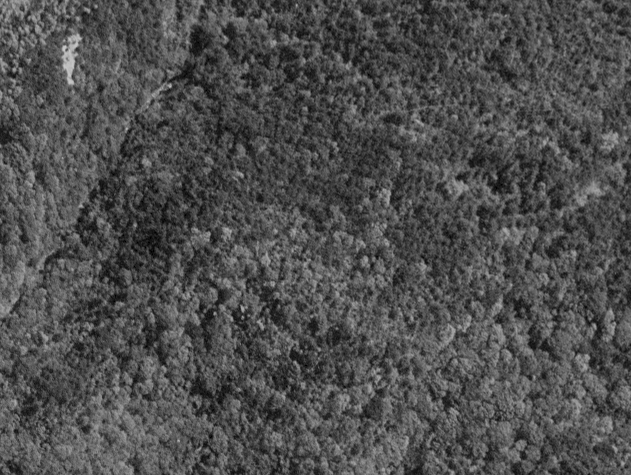
\includegraphics[width=6.2cm]{images/Chapitre1/PoorlyTexturedRGBL.png}
			\end{minipage}%
		}
		\subfigure[Image 2015]{
			\begin{minipage}[t]{0.45\linewidth}
				\centering
				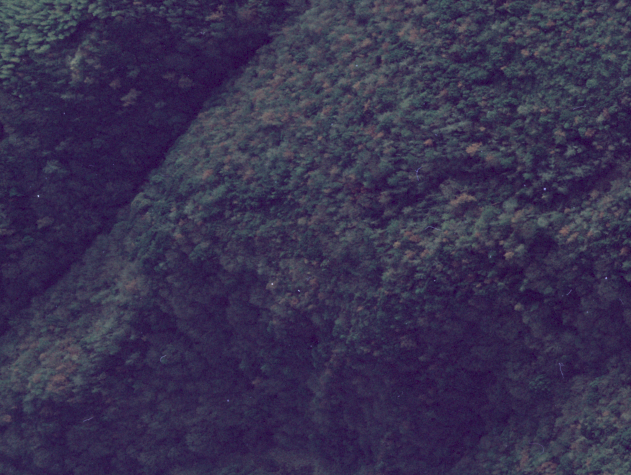
\includegraphics[width=6.2cm]{images/Chapitre1/PoorlyTexturedRGBR.png}
			\end{minipage}%
		}
		\subfigure[\ac{DSM} 1971]{
			\begin{minipage}[t]{0.45\linewidth}
				\centering
				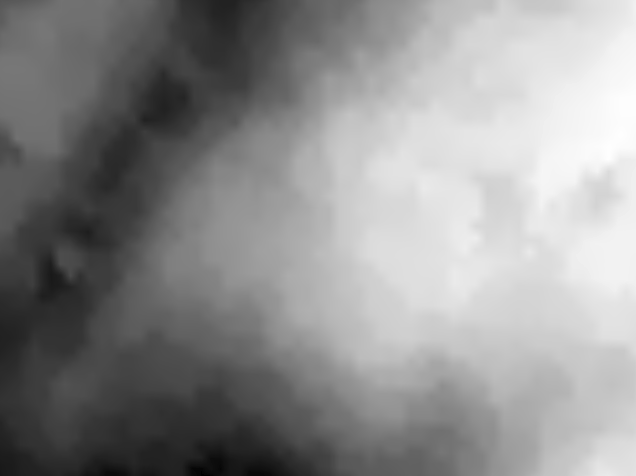
\includegraphics[width=6.2cm]{images/Chapitre1/PoorlyTexturedDSML.png}
			\end{minipage}%
		}
		\subfigure[\ac{DSM} 2015]{
			\begin{minipage}[t]{0.45\linewidth}
				\centering
				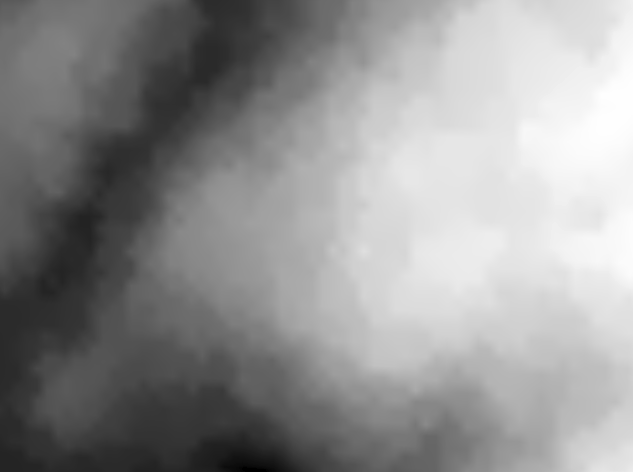
\includegraphics[width=6.2cm]{images/Chapitre1/PoorlyTexturedDSMR.png}
			\end{minipage}%
		}
		\caption{The same vegetation observed in different times. They present non-Lambertian reflection and self similarities, while the \ac{DSM}s are distinctive.}
		\label{PoorlyTextured}
	\end{center}
\end{figure*} 

\subsubsection{Divide and conquer}
%分成CoReg和Precise,前者侧重robust,后者侧重精度.
\begin{figure*}[htbp]
	\begin{center}
		\subfigure[Example of an inter-epoch image pair]{
			\begin{minipage}[t]{1\linewidth}
				\centering
				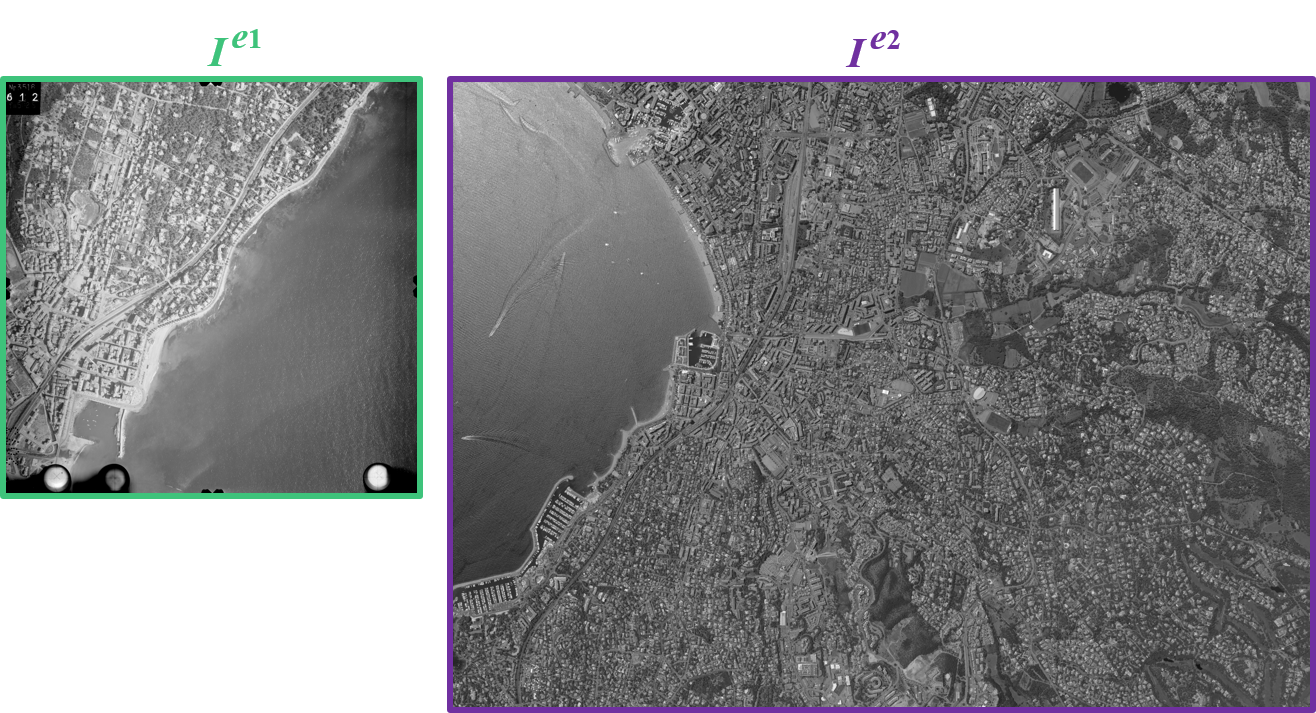
\includegraphics[width=1\columnwidth]{images/Chapitre1/imagepair.png}
			\end{minipage}%
		}
		\subfigure[Rough co-registration]{
			\begin{minipage}[t]{1\linewidth}
				\centering
				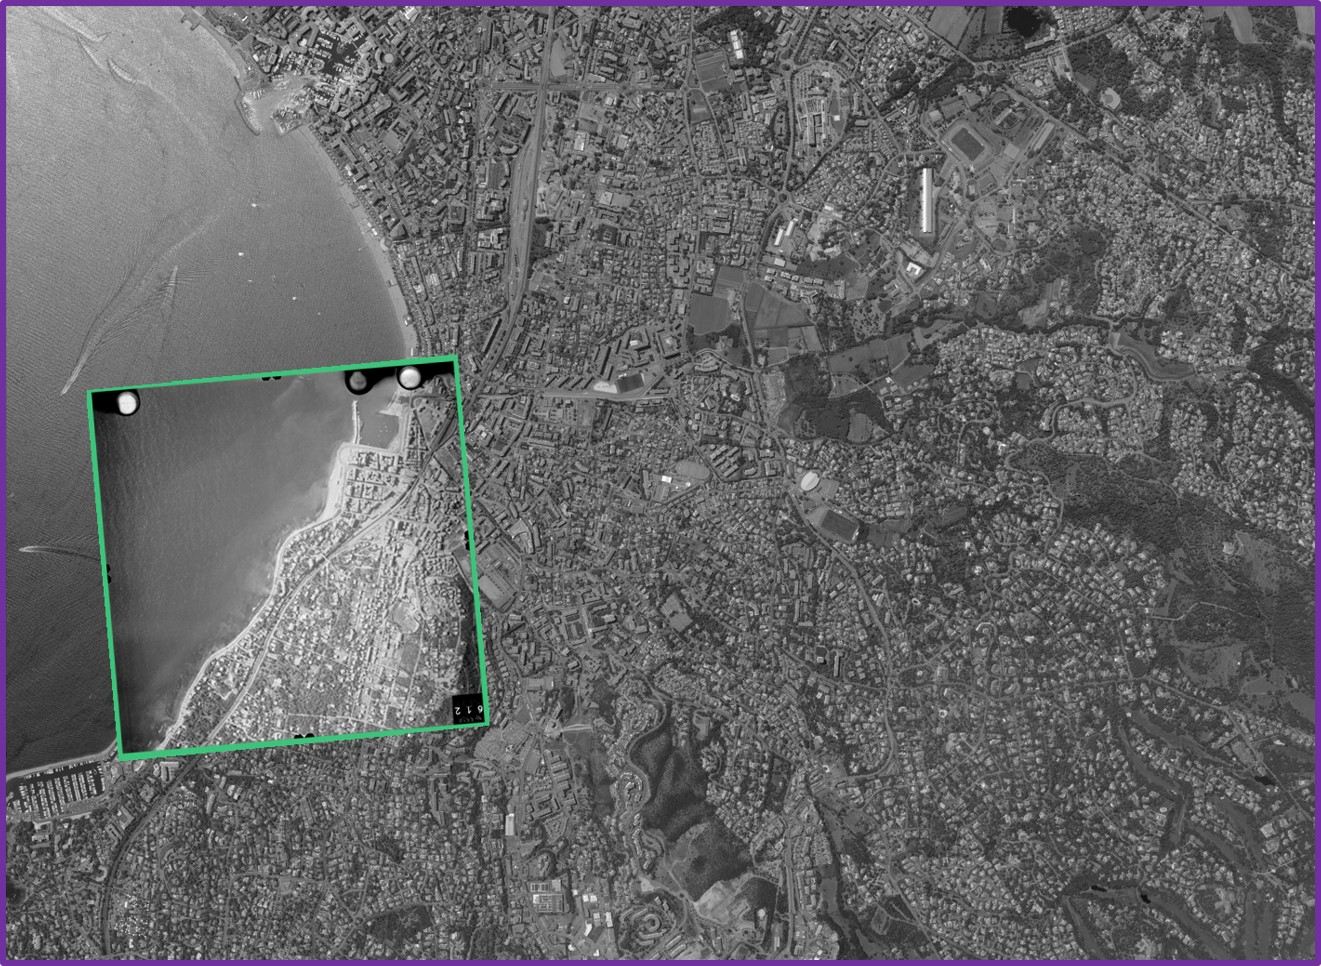
\includegraphics[width=0.68\columnwidth]{images/Chapitre1/CoReg.jpg}
			\end{minipage}%
		}
		\subfigure[Precise matching]{
			\begin{minipage}[t]{1\linewidth}
				\centering
				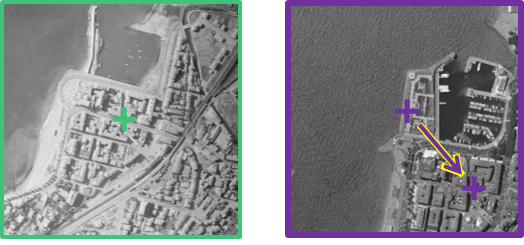
\includegraphics[width=0.55\columnwidth]{images/Chapitre1/Precise.png}
			\end{minipage}%
		}
		\caption{ Rough-to-precise strategy. (a) An example of an inter-epoch image pair to be matched. $I^{e_1}$ and $I^{e_2}$ represents images take at $epoch_1$ and $epoch_2$ individually. (b) Illustration of rough co-registration between $I^{e_1}$ and $I^{e_2}$. As a result, $I^{e_1}$ is roughly but not precisely aligned with $I^{e_2}$. (c) Illustration of precise matching. For keypoints in $I^{e_1}$ (green cross), a location is predicted in $I^{e_2}$ (purple cross) based on rough co-registration, whose neighborhood will be searched to find the precise match (yellow cross).}
		\label{patchexample}
	\end{center}
\end{figure*}

\section{Objective}

\section{Contribution}

\section{Organization of the thesis}
